% -*- mode: LaTeX; mode: TeX-PDF; coding: utf-8  -*-

\label{sec:func_recv}

%%%%%%%%%%%%%%%%%%%%%%%%%%%%%%%%%%%%%%%%%%%%%%%%%%%%%%%%%%%%%%%%%

\subsection*{Описание параллельного вычислительного алгоритма  восстановления данных}

Введём  следующие обозначения:
\begin{itemize}

\item
  $F$  --- массив  известных значений функции $\varphi$
  в узлах крупной сетки;

\item
  $G_{r+\mathbf{2}^n}$ --- массив
  значений аппроксимирующей функции в узлах мелкой сетки,
  вычисленных по формуле~\eqref{eq:recv_common};

\item
  $\Psi_{r+\mathbf{2}^n}$ --- массив  значений ядер В. А. Стеклова порядка $r+\mathbf{2}^n$.

\end{itemize}

%\emph{согласен что плохо, но непонятно какая концепция у нас}

%Учитывая финитность и симметрию ядер В. А. Стеклова
%в массиве $\Psi_{2}$ нужно хранить $N^*$
%значений ядер $\psi_{2}$;
%%на одном интервале крупной сетки;
%в массиве $\Psi_{4}$ нужно хранить $2N^*$
%значений ядер $\psi_{4}$.
%на двух смежных интервалах крупной сетки.

% Учитывая финитность и симметрию ядер В. А. Стеклова
% в массиве $\Psi_{{r+\mathbf{2}^n}}$ достаточно хранить $\overline{r(N+\mathbf{1}^n)/ 2}$
% значений.

% \emph{Сюда можно вставить рисунок 2D ядра 2го порядка для наглядности.
% Выделить ту четвертинку, которую храним.}
Пример ядра порядка $(4,4)$ для $N=(4,4)$ 
представлен на рисунке~\ref{fig:kern_4_4}.

\begin{figure}[h!]
  \centering
  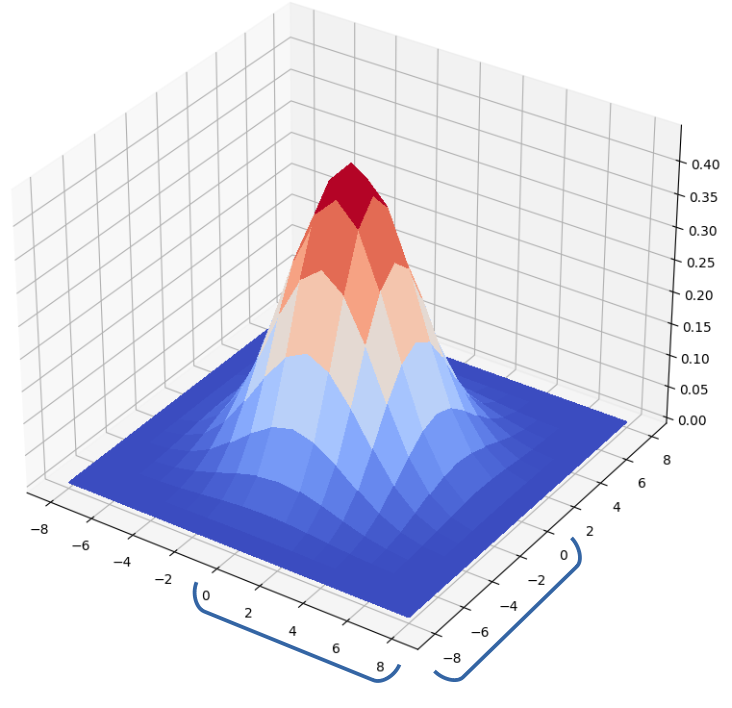
\includegraphics[width=\textwidth
   % ,height
  ]{kern_4_4} 
  \caption{Ядро  порядка $(4,4)$}
  \label{fig:kern_4_4}
\end{figure}
\FloatBarrier


 Далее приведены выражения для формирования
 %элементов
 искомых значений в узлах мелкой сетки.
% %,
% \emph{где $n$ -- количество координат (размерность задачи). --- уже раньше использовали}
%\emph{Итоговая формула, м.б. от массивов вернуться к функциям?}
Пусть $m\in M$, $r/2 \in \mathbb{Z}_+^n$, тогда
\begin{equation}
  \label{eq:nd}
    G_{r+\mathbf{2}^n}[m] = 
    \sum_{i \in  [\mathbf{0}^n:r/2]}\ \sum_{p\in P} 
        F \left[ \left \lfloor {m}/{N} \right \rfloor + ip + s(p)\right]
      \Psi_{r+\mathbf{2}^n}[|m\bmod N - (ip + s(p))N|],
\end{equation}
где $P=\{p\in\mathbb{Z}^n: p_l\in\{-1,1\},\ l=1,\ldots,n\}$, $s(t)=(t+1)/2$
($t\in\mathbb{R}$).

%<$ip$ и $pi$ в ф-ле лучше бы смотрелись в одном порядке, первый вар-т, исправила>

При вычислениях по формуле~\eqref{eq:nd} требуется
%в двумерном случае (2 - операции * и +, 4 части)
%$2 * 4 * \overline{(r/\mathbf{2}^n+\mathbf{1}^n) M}.$
%в общем случае (2 - операции * и +, $2^n$ частей)
$\overline{M}\overline{(r/2+\mathbf{1}^n)} 2^n$
умножений и
$\overline{M}(\overline{(r/2+\mathbf{1}^n)}2^n -1)$
сложений.
%<!!! согласовать (и притащить из этапа 2)> 

% Заметка про этапы индексации.
% \emph{Можно как=то учесть в обозначениях}
% \begin{enumerate}
% \item
%   Лоцировать ячейку в которой находится искомая точка мелкой сетки.
%   Операция $\left \lfloor \frac{m_j}{N_j^*} \right \rfloor$.

% \item
%   Отобразить индекс в координатах всей мелкой сетки на координаты в ячейке.
%   Операция $m_j \bmod N_j^*$.
% \end{enumerate}
  
%%

Заметим, 
что в формуле~\eqref{eq:nd} каждое из произведений известного значения в узле крупной сетки
со значениями ядер в узлах мелкой сетки используется несколько раз
при формировании результатов в нескольких соседних
%интервалах
ячейках 
крупной сетки.
Используя этот факт, можно сократить количество операций. %умножений ((вычислений)).
%С учётом этого факта,
Предложена следующая двухэтапная вычислительная схема.
\begin{enumerate}
\item
  %Вычисление произведений значений ядер в узлах мелкой сетки
  %для каждого узла крупной сетки.
  Вычисление для $k$-го ($k \in [0:K-\mathbf{1}^n]$)
  известного значения функции 
  элементов массива произведений
  $\Pi_r[k,l] = F[k]\Psi_{r+\mathbf{2}^n}[l]$,
  % ($l \in [0:(r/2+\mathbf{1}^n)(N-\mathbf{1}^n)]$). (($(N-\mathbf{1}^n) $ или $N $?))
  ($l \in [0:(r/2+\mathbf{1}^n)N]$). %(($(N-\mathbf{1}^n) $ или $N $?))

Выполняется
%$\overline{K (N(r/2 + \mathbf{1}^n) +\mathbf{1}^n)}$ умножений.
$\overline{K (N(r/2 + \mathbf{1}^n) )}$ умножений.
% ((Да! это для универсальности при попадании в точку крупной сетки
  % -- Правильно ли я понимаю, что $\mathbf{1}^n$ справа учитывает умножения на нули))
\item
  Выбор и суммирование полученных на предыдущем шаге произведений
  для формирования результирующих значений в узлах мелкой сетки.
  
  %Выполняется $r^2M$ сложений.
  %$M$ сложений в первом варианте и
  %$3M$ сложений --- во втором.

  %Выполняется $(2^n-1)  (\overline{(r/2+\mathbf{1}^n)} -1)  \overline{M}$ сложений.
  Выполняется $\overline{M}  (\overline{(r/2+\mathbf{1}^n)}2^n -1)  $ сложений.
%  ((Мне кажется Выполняется $\overline{M}  (\overline{(r/2+\mathbf{1}^n)}2^n -1)  $ сложений.

\end{enumerate}

Таким образом за счёт переиспользования произведений при применении вычислительной схемы
количество умножений сокращается почти в  $2^n$ раз.
%((рисунок подвинуть! $r=(2,2)$!))
%<убрала p и разделитель, тк кратко будет сложно объяснить и непонятно где>
%Иллюстрация при $r=(2,2)$ суммирования по одной координате на рисунке.
Суммирования по одной координате  при $r=(2,2)$ проиллюстрировано на рисунке~\ref{fig:sum_1d}.
\begin{figure}[h!]
  \centering
  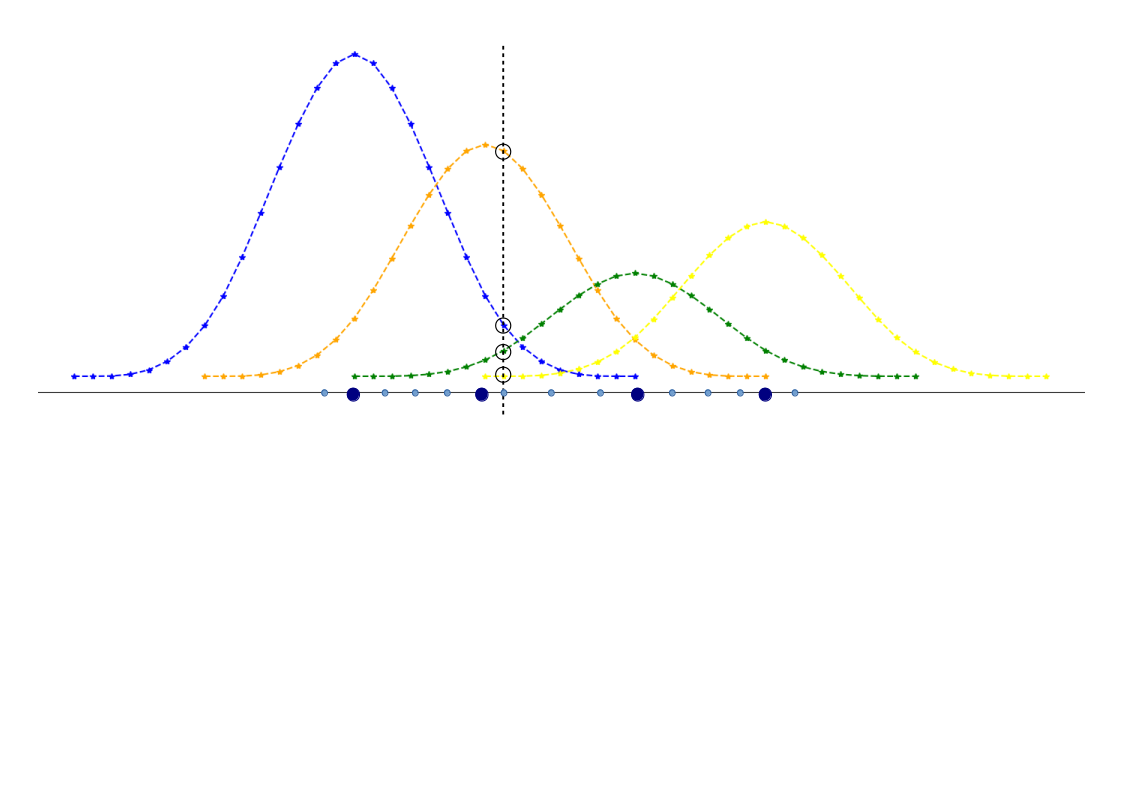
\includegraphics[width=\textwidth,height=7cm]{multi_kern} 
  \caption{пример для одной координаты}
  \label{fig:sum_1d}
\end{figure}
\FloatBarrier


Иллюстрация вычислительной схемы приведена на рисунке~\ref{fig:reg_net}.
\begin{figure}[h!]
  \centering
  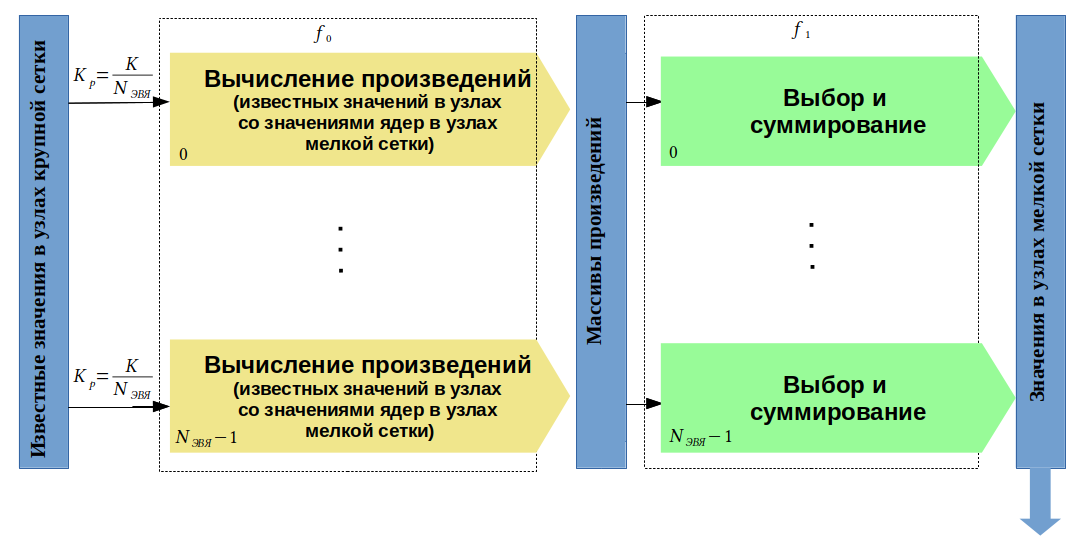
\includegraphics[width=\textwidth,height=7cm]{comp_scheme_steps} 
  \caption{Двухэтапная вычислительная схема}
  \label{fig:reg_net}
\end{figure}
\FloatBarrier


%\subsection*{Программная реализация параллельного вычислительного алгоритма
%  восстановления данных в стандарте Open CL в двумерном случае}

%<Мб всё так отделить реализацию от алгоритма подзаголовком.>
%
%<Не знаю нужны ли подзаголовки по тексту вообще.
%Но пока оставим, могут попросить убрать.
%Например рисунки по требованиям подписываются только Рис.N
%без текстового заголовка, описание только в тексте>
%

Опишем программную реализацию
параллельного вычислительного алгоритма
восстановления данных в стандарте Open CL в двумерном случае.
Из памяти управляющего процессора
в глобальную память вычислителя 
загружаются следующие данные: 
\begin{itemize}
\item
  массив значений в узлах крупной сетки. %размером $K = K_y*K_x$;
\item
  предварительно инициализированный массив значений ядра порядка $r+\mathbf{2}^2$.
  % , вычисленных в $(r/2)^2$ ячейках мелкой сетки.
%((уже было здесь лишнее)):
  % C учётом финитности ядра и его симметричности
  % по   обоим координатам
  % хранить достаточно одну четверть (см. рисунок~\ref{fig:kern_4_4}).
  %Инициализируется предварительно.
\end{itemize}

Результирующие значения в узлах мелкой сетки выгружаются управляющим процессором
из глобальной памяти вычислителя по завершению работы вычислительных ядер на рабочих элементах.
%((Возможно был бы уместен рисунок илл. предыдущее --- это рис.7 (схема) --- можно и тут ссылку))

Программная реализация рассмотренного алгоритма в двухмерном случае
включает в себя 2 вычислительных ядра, соответствующие этапам схемы вычислений.
Первое вычислительное ядро выполняется в рабочем пространстве размером $K$,
для второго ядра удобно выбрать рабочее пространство размером $M$.
Далее приведено описание разработаных вычислительных ядер.
\begin{itemize}
\item
  {\bf kernel prod}

  Выполняется в каждой точке крупной сетки.
  Каждый %вычислительный
  рабочий элемент 
  получает %точку
  значение в точке крупной сетки
  из глобальной памяти по индексу $globalID$. 

  %Размер задачи $K$ (оно же
  %максимальное количество параллельно выполняющихся kernel prod).
  %Размер задачи для этого ядра одномерный (но мб двумерным сделать для наглядности).

  На выходе в глобальной памяти
  формируются массивы произведений в %$r/2$ ((?? -- да, без квадрата, тк это ячеек в штуках!))
  ячейках мелкой сетки,  
  соответствующие каждой точке крупной сетки.
  %(($(r/2)$ --- вектор, не понял и закомментировал))
%Выходная структура данных типа map --- для взаимно однозначного соответствия точка -> массив произведений в ячейках.

  
\item
  {\bf kernel sum}

  Выполняется в каждой точке мелкой сетки. Получает из глобальной памяти массив произведений.
% как используется $globalID$
  % описать как и откуда получаются пр-я аналогично kernel prod
  
  % Суммирует $r$ ближайших по каждой координате к $globalID$ произведений.
  % r и globalID --- это вектора! Разобраться!
  
  
  
  Каждый
  % вычислительный
  рабочий элемент записывает %свою точку
   полученное в соответствии с формулой~\eqref{eq:nd} значение в своей точке мелкой сетки %в   массив
  в глобальную память по индексу $globalID$.
\end{itemize}



%%% Local Variables: 
%%% mode: latex
%%% TeX-master: "paper_func_recv"
%%% End: 


